\documentclass[letterpaper]{article}
\usepackage{aaai}
\usepackage{times}
\usepackage{helvet}
\usepackage{courier}
\usepackage{booktabs}
\usepackage{microtype}
\usepackage{amsmath}
\usepackage{amssymb}
\usepackage{graphicx}
\usepackage{float}
\usepackage{tikz}
\usepackage{fontawesome5}
\usetikzlibrary{arrows.meta,positioning,fit,backgrounds,calc,shapes.geometric}
\definecolor{panelA}{HTML}{EAF2EA}
\definecolor{panelB}{HTML}{EAF0FA}
\definecolor{boxedge}{HTML}{6B7280}
\definecolor{accentA}{HTML}{2E7D5B}
\definecolor{accentB}{HTML}{2F5BAA}
\definecolor{subcap}{HTML}{4B5563}
\frenchspacing
\setlength{\pdfpagewidth}{8.5in}
\setlength{\pdfpageheight}{11in}
\pdfinfo{
/Title (bioMoR: Biology-Guided Mixture-of-Recursions for Efficient and Interpretable Genomic Learning)
/Author (Anonymous Submission)
/Keywords (single-cell genomics, multi-omics, transformers, parameter efficiency, marker genes, recursive computation, learned gene graph)
}
\setcounter{secnumdepth}{1}

\title{bioMoR: Biology-Guided Mixture-of-Recursions for Efficient and Interpretable Genomic Learning}
\author{Anonymous Submission}

\begin{document}
\maketitle


\begin{abstract}
    \begin{quote}
        Transformer models for transcriptomic analysis typically allocate equal computation to all genes or pathways, although only a subset is biologically informative. We propose \textbf{bioMoR}, a biology-guided adaptive recursive framework that incorporates gene–gene or Reactome pathway–pathway interactions into both embedding refinement and token routing. bioMoR compresses the input into a small set of interpretable marker or pathway tokens, applies one weight-shared block recursively, and combines data-driven and biology-prior scores to allocate deeper computation to informative tokens while freezing less relevant ones. The framework supports both expert-choice and token-choice routing and reuses shared recursion blocks for parameter efficiency. Across eight single-cell and six multi-omics benchmarks under a unified 5-fold cross-validation protocol, bioMoR improves average macro-F1 by up to $7.1$ points over the strongest biology-agnostic Mixture-of-Recursions baseline ($68.2\%$ vs.\ $61.1\%$), while using $75\%$ fewer parameters (one shared block in place of four independent layers) and up to $58\%$ fewer FLOPs. Through degree-matched random-graph controls and an injection-site ablation we further isolate \emph{where} biology should enter: a rigid hand-built prior injected into the router fails to separate from chance, whereas a \emph{learned} low-rank interaction graph helps at \emph{both} injection sites---smoothing the token embeddings and steering depth allocation through a zero-initialised graph-convolution router---and injecting biology at both sites jointly is best. Adaptive recursion depth additionally provides an interpretable, per-token measure of allocated computation. These results demonstrate that a learned interaction graph, injected at both the embedding and routing sites and combined with parameter-efficient adaptive recursion, offers an effective, efficient, and interpretable framework for transcriptomic learning.
    \end{quote}
\end{abstract}

\section{Introduction}
\label{sec:introduction}
\begin{figure*}[t]
\centering

\includegraphics[width=0.85\linewidth]{figs/overview.pdf}
\caption{\footnotesize\textbf{Overview of bioMoR.} Inputs are embedded and refined by a
learned interaction graph; a selector keeps the top-$M$ marker/pathway tokens; a bio-router
sends selected tokens through further weight-shared recursion (adaptive depth). One pipeline
serves single-cell and multi-omics.}
\label{fig:overview}
\end{figure*}

\begin{table}[t]
\centering
\setlength{\tabcolsep}{3pt}
\resizebox{\linewidth}{!}{%
\begin{tabular}{lccccccc}
\toprule
& Pre- & Efficient & Multi- & Biology & Adaptive & Shared & Learned \\
Method & trained & tokens & omics & prior & depth & recursion & graph \\
\midrule
\multicolumn{8}{l}{\emph{Genomic / single-cell transformers}}\\
scGPT \cite{cui2024scgpt}                 & \checkmark & -- & -- & -- & -- & -- & -- \\
Geneformer \cite{theodoris2023transfer}   & \checkmark & -- & -- & -- & -- & -- & -- \\
scBERT \cite{scbert2022}                  & \checkmark & \checkmark & -- & -- & -- & -- & -- \\
scFoundation \cite{hao2024large}          & \checkmark & \checkmark & -- & -- & -- & -- & -- \\
UCE \cite{uce2026}                        & \checkmark & -- & -- & -- & -- & -- & -- \\
xTrimoGene \cite{xtrimogene2023}          & \checkmark & \checkmark & -- & -- & -- & -- & -- \\
tGPT \cite{tgpt2023}                      & \checkmark & -- & -- & -- & -- & -- & -- \\
scMulan \cite{scmulan2024}                & \checkmark & -- & -- & -- & -- & -- & -- \\
CellFM \cite{cellfm2025}                  & \checkmark & \checkmark & -- & -- & -- & -- & -- \\
LangCell \cite{langcell2024}              & \checkmark & -- & -- & -- & -- & -- & -- \\
Nicheformer \cite{nicheformer2024}        & \checkmark & -- & \checkmark & -- & -- & -- & -- \\
scRCL \cite{peng2026scrcl}                & \checkmark & -- & -- & -- & -- & -- & -- \\
GeneIncr.\ \cite{qi2026geneincremental}   & \checkmark & -- & -- & -- & -- & -- & -- \\
GeneMamba \cite{genemamba2024}            & \checkmark & \checkmark & -- & -- & -- & -- & -- \\
BMFM-RNA \cite{bmfmrna2025}               & \checkmark & -- & -- & -- & -- & -- & -- \\
CellPLM \cite{cellplm2024}                & \checkmark & -- & -- & \checkmark & -- & -- & -- \\
GeneCompass \cite{genecompass2024}        & \checkmark & -- & -- & \checkmark & -- & -- & -- \\
scMoFormer \cite{scmoformer2023}          & -- & -- & \checkmark & \checkmark & -- & -- & -- \\
GenoHoption \cite{cheng2024genohoption}   & \checkmark & -- & -- & \checkmark & -- & -- & -- \\
\addlinespace
\multicolumn{8}{l}{\emph{Adaptive-compute transformers}}\\
MoD \cite{raposo2024mixture}              & -- & -- & -- & -- & \checkmark & -- & -- \\
MoR \cite{bae2025mixture}                 & -- & -- & -- & -- & \checkmark & \checkmark & -- \\
\addlinespace
\multicolumn{8}{l}{\emph{Biology-structured models}}\\
genomap \cite{islam2023cartography}       & -- & -- & -- & \checkmark & -- & -- & -- \\
scTransformer \cite{sctransformer2024}    & -- & -- & -- & \checkmark & -- & -- & -- \\
DOGMA \cite{dogma2024}                    & -- & -- & \checkmark & \checkmark & -- & -- & -- \\
GATTACA \cite{mizera2026gattaca}          & -- & -- & -- & \checkmark & -- & -- & -- \\
P-NET/PATH \cite{elmarakeby2021biologically,howlader2026graph} & -- & \checkmark & \checkmark & \checkmark & -- & -- & -- \\
Pathformer \cite{pathformer2023}          & -- & -- & \checkmark & \checkmark & -- & -- & -- \\
scBiGNN \cite{scbignn2023}                & -- & -- & -- & \checkmark & -- & -- & \checkmark \\
ORBIT \cite{orbit2026}                    & -- & \checkmark & -- & \checkmark & -- & -- & -- \\
\midrule
\textbf{bioMoR (ours)}                    & -- & \checkmark & \checkmark & \checkmark & \checkmark & \checkmark & \checkmark \\
\bottomrule
\end{tabular}}
\caption{\footnotesize\textbf{Positioning bioMoR against recent models.} Columns are design
axes; \checkmark{} = built-in. bioMoR uniquely unifies a learned interaction graph with
adaptive weight-shared recursion, token compression, and multi-omics.}
\label{tab:positioning}
\end{table}


Recent advances in high-throughput sequencing technologies have enabled the measurement of thousands of molecular features at single-cell and multi-omics resolution, providing unprecedented opportunities to study cellular heterogeneity, disease mechanisms, and precision medicine \cite{luecken2019current,stuart2019integrative,hasin2017multiomics}. Transformer-based architectures have recently become a powerful paradigm for modeling these high-dimensional genomic data because self-attention can capture long-range dependencies among genes and pathways. Foundation models such as Geneformer, scBERT, scGPT, and scFoundation have demonstrated remarkable performance across a wide range of transcriptomic tasks, including cell-type annotation, perturbation prediction, and representation learning \cite{theodoris2023transfer,yang2022scbert,cui2024scgpt,hao2024large}.

Despite these advances, conventional transformers remain computationally expensive for genomic data. Self-attention scales quadratically with the number of input tokens, while stacking multiple transformer layers further increases memory and parameter complexity \cite{vaswani2017attention}. More importantly, existing transformer architectures allocate the same amount of computation to every gene or pathway, although only a small subset is typically informative for a specific biological condition, cell type, or disease phenotype. This uniform computation is inconsistent with the sparse and hierarchical nature of biological systems.

Recent work has explored two complementary directions to improve transformer efficiency. Efficient-attention methods, including Linformer, Performer, and Nyströmformer, reduce the computational complexity of self-attention through low-rank or kernel approximations \cite{wang2020linformer,choromanski2021performer,xiong2021nystromformer}. Separately, adaptive computation methods, including Adaptive Computation Time, Mixture-of-Experts, Mixture-of-Depths, and the recently proposed Mixture-of-Recursions (MoR), allocate different amounts of computation to different inputs by dynamically routing tokens through recursive transformer blocks \cite{graves2016act,shazeer2017moe,raposo2024mixture,bae2025mixture}. Although these approaches substantially improve computational efficiency, their routing decisions are entirely data-driven and do not exploit well-established biological relationships among genes or pathways.

In parallel, numerous studies have demonstrated the value of incorporating biological priors into deep learning models. Marker-gene databases such as PanglaoDB and CellMarker organize experimentally validated cell-type markers \cite{franzen2019panglaodb,hu2023cellmarker}, while pathway databases such as Reactome provide curated gene--pathway and pathway--pathway relationships \cite{gillespie2022reactome}. Biology-aware architectures, including P-NET, Genomap, and GenoHoption, further show that integrating prior biological knowledge improves interpretability and predictive performance \cite{elmarakeby2021biologically,islam2023cartography,cheng2024genohoption}. However, existing approaches use biological knowledge primarily for feature construction or network design rather than for determining how computational resources should be allocated during inference.

In this work, we introduce \textbf{bioMoR} (\textbf{bio}logy-guided \textbf{M}ixture-\textbf{o}f-\textbf{R}ecursions), a biology-guided adaptive recursive transformer for transcriptomic learning. Unlike existing recursive transformers, bioMoR incorporates gene--gene or Reactome pathway--pathway interaction knowledge into both representation learning and adaptive routing. Biological interaction networks first refine gene or pathway embeddings through graph-based propagation, and the resulting biological prior is subsequently combined with the data-driven routing score to determine which marker tokens receive deeper recursive computation. Consequently, bioMoR allocates computation according to both the observed sample and its underlying biological context. The proposed framework naturally supports both expert-choice and token-choice routing while preserving the parameter efficiency of shared recursive transformer blocks.

We evaluate bioMoR on eight single-cell transcriptomic datasets and six multi-omics benchmarks (fourteen in total) under a unified 5-fold cross-validation protocol. On average, bioMoR outperforms Vanilla Transformers, Recursive Transformers, and biology-agnostic Mixture-of-Recursions under both expert-choice and token-choice routing: its best configuration reaches an average macro-F1 of \textbf{68.2\%}, improving over Vanilla Transformers (60.1\%), Recursive Transformers (60.4\%), and MoR (61.1\%) by roughly $7$--$8$ points, while using approximately $4\times$ fewer transformer parameters and reducing recursive FLOPs by up to 58\%. A controlled analysis further isolates \emph{where} biology helps: a rigid hand-built prior injected into the router fails, whereas a \emph{learned} interaction graph is effective at both the embedding and routing sites---smoothing token embeddings and steering depth allocation through a zero-initialised graph-convolution router---and injecting it at both sites jointly is best.

Our contributions are summarized as follows:

\begin{itemize}
    \item We propose \textbf{bioMoR}, a biology-guided adaptive recursive transformer that unifies marker/pathway token compression, weight-shared recursion, and adaptive per-token depth for both single-cell and multi-omics data.

    \item We introduce a \textbf{Bio Router} together with a \emph{learned} low-rank gene--gene graph that smooths the input before token selection, and study both carefully with degree-matched random-graph controls and warm-start stress tests.

    \item Through this controlled study we identify a \emph{learned} interaction graph---not a fixed biological prior---as the decisive driver, and show it helps at \emph{both} the embedding and routing sites, an honest negative-and-positive result that clarifies where biological structure helps.

    \item On fourteen genomic benchmarks under a unified 5-fold cross-validation protocol, bioMoR improves average predictive performance over Vanilla Transformers, Recursive Transformers, and biology-agnostic MoR while substantially reducing parameters and FLOPs, and we report an honest comparison against strong classical baselines.
\end{itemize}

\paragraph{Positioning against recent biology-aware models.}
bioMoR sits among a fast-growing set of pathway- and graph-aware genomic models
(Table~\ref{tab:positioning}). Closest on the multi-omics side is PATH
\cite{howlader2026graph}, which conditions gene embeddings on patient-specific
alterations and refines a pathway graph inside attention on P-NET-style cohorts;
Pathformer \cite{pathformer2023} likewise injects pathway structure into attention for
multi-omics classification. On the single-cell side, scBiGNN \cite{scbignn2023} learns
gene--gene structure through a bilevel graph network, and ORBIT \cite{orbit2026} operates
on pathway/program tokens with an asymmetric objective, while GeneMamba
\cite{genemamba2024} pursues efficiency through a linear-time state-space backbone rather
than adaptive recursion. Two points distinguish our work. First, unlike these models
bioMoR makes computation \emph{adaptive per token} through weight-shared recursion, so its
parameter/FLOP efficiency and its interpretable depth signal arise from the same
mechanism. Second, our controls speak directly to a recent cautionary literature: whereas
DOGMA \cite{dogma2024} emphasizes deterministic prior-driven structure, recent
re-evaluations \cite{pathwayprior2025} argue that sparsity---not biological
correctness---explains much of the benefit attributed to pathway priors. Our
degree-matched random-graph controls, and our finding that a \emph{learned} graph beats a
fixed biological one, corroborate that view within an adaptive-recursion setting. We do
not run PATH or scBiGNN head-to-head here---a limitation we return to in the discussion---but
position bioMoR against them along these axes.

\section{Method and Experiments}

\paragraph{Token interface (markers and pathways).}
bioMoR turns the input into $M\ll N$ interpretable tokens before any quadratic
attention. For single-cell expression these are \emph{learned marker} tokens from the
cross-attention router. For bulk multi-omics they are fixed \emph{Reactome pathway}
tokens: a sparse gene$\to$pathway membership pools each pathway's per-gene channels
(mean pooling for dense assays such as copy-number and expression; burden/sum pooling
for sparse binary mutation), so every token is a named pathway. Both feed the same
recursive stack, and on top of token selection we study the full design space --
token count, weight-sharing scheme (Cycle / Sequence / Middle-Cycle / Middle-Sequence,
from one shared block to $K$ independent ones), expert- vs token-choice depth routing,
reuse of the first-step attention key/value across recursions, and warm-starting the
shared block from a fixed-depth model.


\subsection{Overview}
Let $x \in \mathbb{R}^{N}$ be the expression vector of a cell over $N$ genes. bioMoR
maps $x$ to cell-type logits through five stages: gene embedding, learnable marker
selection, marker-anchored compression, biology-informed recursive shared
transformation with marker refinement, and a pooled classifier
(Figure~\ref{fig:overview}).

\subsection{Gene Embedding}
Each gene $i$ is embedded as the sum of a learned identity vector
$\mathbf{e}_i \in \mathbb{R}^d$ and a projection of its scalar expression,
$\mathbf{t}_i = \mathbf{e}_i + \mathbf{W}_v\, x_i$, following the gene-plus-value
scheme of \cite{cui2024scgpt,theodoris2023transfer}. This is linear in $N$ and runs
over all genes before any compression.

\subsection{Cross-Attention Marker Router}
We identify markers with a cross-attention \emph{router}. We maintain $M$ learnable
marker queries $\mathbf{q}_m \in \mathbb{R}^{d}$; each attends over the genes through a
shared key projection $\mathbf{k}_i = \mathbf{W}_k \mathbf{e}_i$, giving selection
weights
$\mathbf{w}_m = \mathrm{softmax}\big(\mathbf{q}_m \mathbf{K}^{\top}/(\tau\sqrt{d})\big)$
over \emph{all} $N$ genes, with temperature $\tau$ annealed from soft to peaked.
Because the softmax spans all genes, gradients reach every gene, so a query can
migrate to an informative gene it did not initially favour, the property hard top-$k$
routing lacks. Two ingredients are essential: the all-gene softmax, and a
\emph{peaked initialisation} that points each query at a distinct gene's key, so
training starts at random-selection quality rather than a uniform average of all
genes. At inference each query collapses to its arg-max gene
$g_m = \arg\max_i \mathbf{q}_m^{\top}\mathbf{k}_i$, giving discrete, interpretable
markers and $\mathcal{O}(M^2 d)$ attention. As alternatives we consider the Concrete
selector \cite{balin2019concrete,jang2017categorical} and fixed variance- and
random-selected panels.

\subsection{Marker Tokens}
Each query produces one marker token combining the (soft-)selected gene identity and
expression,
$\mathbf{c}_m = (\mathbf{w}_m^{\top}\mathbf{E}) + \mathbf{W}_v\,(\mathbf{w}_m^{\top}\mathbf{x})$,
where $\mathbf{E}\in\mathbb{R}^{N\times d}$ are the gene-identity embeddings. The two
contributions are placed on a common scale by the pre-norm LayerNorm at the entry of
the shared block (Sec.~\ref{sec:rec}).

\subsection{Weight-Shared Adaptive Recursion (from MoR)}
\label{sec:rec}
We reuse the Mixture-of-Recursions backbone \cite{bae2025mixture}: a \emph{single} pre-norm
block $f_\theta$ is applied up to $K$ times, $\mathbf{H}^{(t+1)}=f_\theta(\mathbf{H}^{(t)})$,
$\mathbf{H}^{(0)}=\mathbf{C}$, tying all depth-wise parameters
\cite{dehghani2019universal,lan2020albert} so the stack's size is independent of $K$. Depth
is \emph{adaptive per token} (Fig.~\ref{fig:mor}): \emph{expert-choice} keeps the
top-$\lceil c_t M\rceil$ tokens each step (our headline) and \emph{token-choice} lets each
token self-gate with a Switch-style load-balancing loss \cite{shazeer2017outrageously}; both
share $f_\theta$ and reduce to fixed-depth recursion when routing is off. A token's
surviving-step count is its interpretable \emph{recursion depth} $d_m\in\{0,\dots,K\}$---an
architecture-intrinsic compute-allocation score. A per-token gate recomputed from the updated
embeddings, $g^{(t)}_m=\sigma(\mathrm{MLP}_r(\mathbf{H}^{(t)}_m))$, refines markers between
steps.

\begin{figure*}[t]
\centering
\IfFileExists{figs/fig2_depth.pdf}{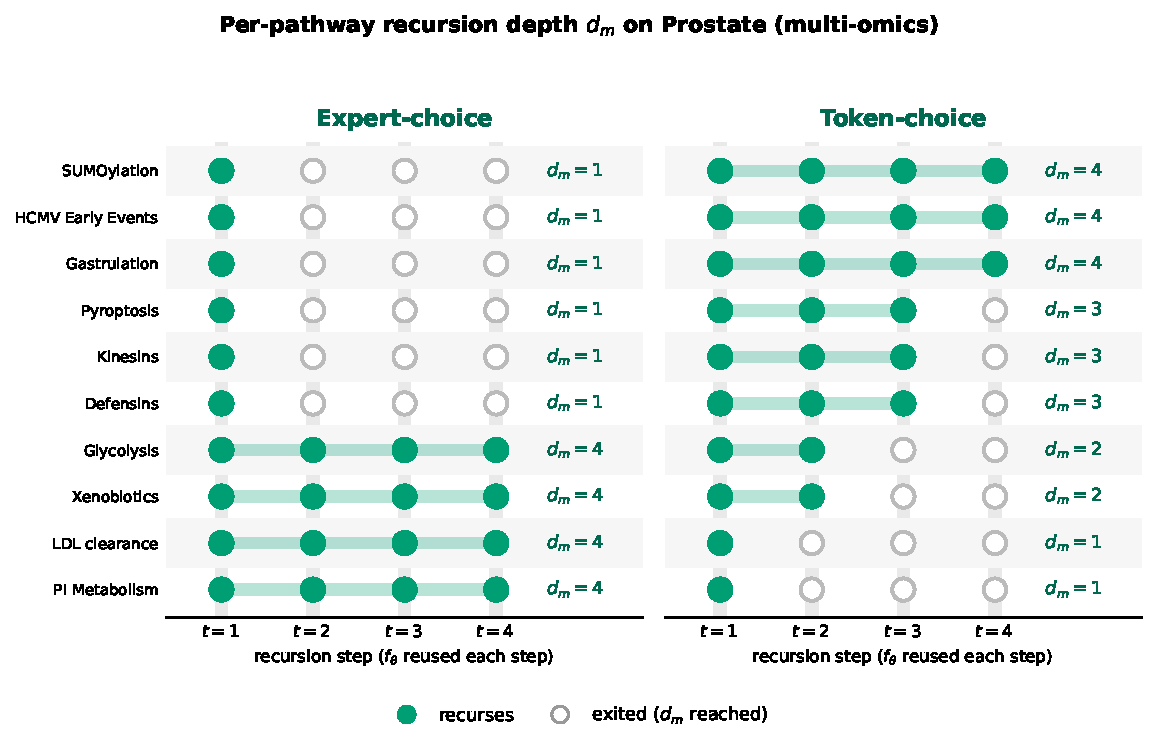
\includegraphics[width=0.90\textwidth]{figs/fig2_depth.pdf}}{\emph{(real per-pathway depth panels render here once the run lands)}}
\caption{\textbf{Two routing modes assign per-pathway depth $d_m$} (real Prostate tokens;
$\bullet$ recurses, $\circ$ exited; the block $f_\theta$ is reused up to $K{=}4$, so depth
adds no parameters). Expert-choice fixes capacity per step; token-choice lets each pathway
self-gate its depth.}
\label{fig:mor}
\end{figure*}

\subsection{Biology-Informed Routing}
\label{sec:biorouter}
The backbone so far---embedding, marker/pathway compression, weight-shared recursion, and
expert-/token-choice depth routing---follows Mixture-of-Recursions and recursive transformers
\cite{bae2025mixture,dehghani2019universal,lan2020albert}. bioMoR's contribution is to inject
a \emph{learned} biological interaction graph at \emph{two} sites of this backbone: the depth
\emph{router} and the token \emph{embedding}. At the router, the expert-choice depth logit for
token $m$ at step $t$ takes the form
\begin{equation}
\tilde r^{(t)}_m \;=\; \underbrace{\tfrac{1}{\tau}\,\mathbf{w}_r^{\top}\mathbf{H}^{(t)}_m}_{\text{data-driven (learned)}}
\;+\; \underbrace{\beta_t\,\pi_m}_{\text{biological prior}},
\label{eq:biorouter}
\end{equation}
and the keep/drop top-$\lceil c_t M\rceil$ and the gate
$g^{(t)}_m=\sigma(\tilde r^{(t)}_m)$ run exactly as before, so the recursion-depth
definition is unchanged but now reflects prior and data together. This is the same
loss-free additive-bias slot used by Switch routing \cite{shazeer2017outrageously},
except the bias is a per-gene \emph{biological} score, not a load-balancing scalar.

\paragraph{Site 1 (router): a zero-initialised graph-convolution residual.}
A first attempt sets $\pi_m$ to a fixed network centrality (z-scored eigenvector centrality
of the label-free co-expression / Reactome graph) and adds $\beta_t\pi_m$ in
Eq.~\ref{eq:biorouter}. This is a \emph{negative} result: the fixed prior does not separate
from a degree-matched random control and can pin the router to a bad operating point
(Sec.~\ref{sec:interaction}). We therefore replace it with a \emph{learned} residual---the
router message-passes over the row-normalised token graph $\mathbf{A}$ (below) and adds
$\sigma(\gamma_t)\,\mathrm{MLP}\big([\mathbf{A}\mathbf{H}^{(t)},\,\mathbf{H}^{(t)}-\mathbf{A}\mathbf{H}^{(t)}]\big)_m$
to the depth logit, with the MLP output \emph{zero-initialised} so the term begins as a
no-op and can only learn to help, never collapsing routing the way the fixed prior does.

\paragraph{The shared learned graph and Site 2 (embedding).}
Both sites read one \emph{learned} low-rank graph. We attach an embedding
$\mathbf{E}\in\mathbb{R}^{M\times r}$ ($r{=}16$) whose row-cosine similarity is the affinity
$\mathbf{A}=\tilde{\mathbf{E}}\tilde{\mathbf{E}}^{\top}$,
$\tilde{\mathbf{E}}=\mathrm{normalize}(\mathbf{E})$, warm-started from the co-expression graph
(single cell) or the \emph{provided} Reactome pathway$\to$pathway adjacency
(multi-omics, \texttt{adjacency\_matrix.csv}) and then refined end-to-end so it is
discriminative, not merely centrality-maximal. At the embedding site we smooth the tokens
along it, $\mathbf{c}\leftarrow(1-\lambda)\mathbf{c}+\lambda\,(\mathbf{c}\tilde{\mathbf{E}})\tilde{\mathbf{E}}^{\top}$
(learned $\lambda$, low-rank $\mathcal{O}(Mr)$), so its $r$ latent factors act as gene/pathway
programs that denoise each token toward its program consensus. Injecting the graph at
\emph{both} sites is bioMoR; the injection-site ablation (Table~\ref{tab:injection}) shows
the two are complementary and jointly best.

\subsection{Training Objective}
We minimise a composite loss
$\mathcal{L} = \mathcal{L}_{\mathrm{task}} + \lambda\mathcal{L}_{\mathrm{marker}}
+ \gamma\mathcal{L}_{\mathrm{div}} + \zeta\mathcal{L}_{z} + \eta\mathcal{L}_{\mathrm{bal}}$,
where $\mathcal{L}_{\mathrm{task}}$ is class-weighted cross-entropy (inverse-frequency
weights on the train split); $\mathcal{L}_{\mathrm{marker}}$ is the cross-entropy of
an auxiliary linear classifier fed only the pre-recursion cluster tokens, forcing the
marker head to select task-sufficient genes;
$\mathcal{L}_{\mathrm{div}}$ is the off-diagonal energy of the normalised marker Gram
matrix (prevents marker collapse); $\mathcal{L}_{z}$ is the router logit $z$-loss; and
$\mathcal{L}_{\mathrm{bal}}$ is the Switch load-balancing term
\cite{shazeer2017outrageously} for token-choice routing (expert-choice is balanced by
construction). Unless noted $\lambda{=}0.1$, $\gamma{=}0.05$, $\zeta{=}10^{-3}$,
$\eta{=}0.1$; $\tau$ anneals geometrically from $1$ to $0.1$ and each router query is
peak-initialised.

% ============================================================================
% CV5 RESULTS — NATIVE LaTeX tables under the unified 5-fold cross-validation
% protocol. The three \input fragments (cv5_{main,scaling,ablation}_table.tex) are
% regenerated from results_cv5/ by build_cv5_tex.py on every refresh cycle, and the
% paper is recompiled, so cells fill in real time as folds finish ("run..." = pending).
% They SUPERSEDE the pre-CV5 tables archived in archive/paper_pre_cv5_2026-07-13/.
% ============================================================================
\begin{table*}[t]
\centering
\IfFileExists{cv5_main_table.tex}{\resizebox{\textwidth}{!}{%
\begin{tabular}{l l c c c c c c c c c c c c c c c c c}
\toprule
 & & & & & \multicolumn{8}{c}{Single-cell macro-F1 $\uparrow$} & \multicolumn{5}{c}{Multi-omics macro-F1 $\uparrow$} & \\
\cmidrule(lr){6-13}\cmidrule(lr){14-18}
Model & Type & $N_R$ & Param & FLOPs & Bar & Lun & Mur & Oes & Seg & Spl & Tce & Xin & Pro & BL & ST & PM & PC & Avg \\
\midrule
Vanilla & -- & 4 & 300K & 1.00$\times$ & 61.0{\scriptsize$\pm$8.5} & 72.5{\scriptsize$\pm$2.5} & 80.2{\scriptsize$\pm$4.3} & 58.7{\scriptsize$\pm$4.2} & 62.5{\scriptsize$\pm$11.2} & 48.3{\scriptsize$\pm$3.7} & 52.1{\scriptsize$\pm$3.5} & 74.0{\scriptsize$\pm$12.1} & 66.8{\scriptsize$\pm$9.4} & 40.6{\scriptsize$\pm$5.8} & 44.5{\scriptsize$\pm$7.5} & 41.2{\scriptsize$\pm$2.3} & 94.2{\scriptsize$\pm$1.7} & 60.1{\scriptsize$\pm$6.6} \\
\midrule
Recursive & -- & 2 & 75K & 0.50$\times$ & 65.6{\scriptsize$\pm$2.8} & 71.7{\scriptsize$\pm$2.8} & 79.8{\scriptsize$\pm$6.5} & 57.3{\scriptsize$\pm$2.9} & 65.8{\scriptsize$\pm$4.4} & 48.8{\scriptsize$\pm$2.3} & 53.0{\scriptsize$\pm$2.0} & 68.2{\scriptsize$\pm$2.4} & 66.2{\scriptsize$\pm$13.4} & 41.4{\scriptsize$\pm$1.3} & 46.0{\scriptsize$\pm$3.4} & 40.8{\scriptsize$\pm$2.4} & 94.6{\scriptsize$\pm$2.7} & 60.4{\scriptsize$\pm$4.0} \\
 & -- & 3 & 75K & 0.75$\times$ & 67.1{\scriptsize$\pm$8.7} & 72.7{\scriptsize$\pm$2.0} & 78.7{\scriptsize$\pm$4.9} & 57.5{\scriptsize$\pm$2.1} & 64.5{\scriptsize$\pm$3.1} & 49.4{\scriptsize$\pm$3.3} & 49.8{\scriptsize$\pm$4.4} & 67.8{\scriptsize$\pm$7.3} & 63.2{\scriptsize$\pm$7.6} & 43.2{\scriptsize$\pm$6.2} & 45.7{\scriptsize$\pm$3.7} & 38.9{\scriptsize$\pm$1.2} & 94.4{\scriptsize$\pm$1.8} & 60.0{\scriptsize$\pm$4.8} \\
 & -- & 4 & 75K & 1.00$\times$ & 65.9{\scriptsize$\pm$2.7} & 72.9{\scriptsize$\pm$2.9} & 75.8{\scriptsize$\pm$4.1} & 56.9{\scriptsize$\pm$4.3} & 61.4{\scriptsize$\pm$7.3} & 49.4{\scriptsize$\pm$3.4} & 50.5{\scriptsize$\pm$3.5} & 72.2{\scriptsize$\pm$5.2} & 65.3{\scriptsize$\pm$10.0} & 40.2{\scriptsize$\pm$1.1} & 43.2{\scriptsize$\pm$6.0} & \textbf{42.1{\scriptsize$\pm$1.6}} & 96.3{\scriptsize$\pm$1.1} & 59.4{\scriptsize$\pm$4.6} \\
\midrule
\textbf{MoR (general)} & Expert & 2 & 75K & 0.42$\times$ & 58.0{\scriptsize$\pm$6.1} & 72.9{\scriptsize$\pm$1.7} & 72.3{\scriptsize$\pm$2.9} & 57.0{\scriptsize$\pm$3.5} & 65.0{\scriptsize$\pm$6.2} & 51.7{\scriptsize$\pm$1.4} & 50.6{\scriptsize$\pm$4.9} & 68.0{\scriptsize$\pm$8.3} & 71.2{\scriptsize$\pm$11.8} & 39.7{\scriptsize$\pm$12.3} & 49.7{\scriptsize$\pm$6.3} & 37.9{\scriptsize$\pm$2.0} & 94.9{\scriptsize$\pm$1.7} & 59.6{\scriptsize$\pm$5.9} \\
 & Expert & 3 & 75K & 0.59$\times$ & 61.6{\scriptsize$\pm$2.3} & 74.2{\scriptsize$\pm$1.7} & 69.3{\scriptsize$\pm$7.2} & 58.4{\scriptsize$\pm$3.6} & 60.7{\scriptsize$\pm$6.9} & 47.5{\scriptsize$\pm$3.0} & 52.3{\scriptsize$\pm$2.4} & 65.7{\scriptsize$\pm$7.5} & 63.4{\scriptsize$\pm$12.3} & 38.0{\scriptsize$\pm$8.0} & 42.3{\scriptsize$\pm$4.4} & 37.7{\scriptsize$\pm$2.2} & \textbf{96.4{\scriptsize$\pm$1.2}} & 57.6{\scriptsize$\pm$5.4} \\
 & Expert & 4 & 75K & 0.76$\times$ & 68.9{\scriptsize$\pm$3.7} & 72.3{\scriptsize$\pm$2.7} & 74.8{\scriptsize$\pm$4.7} & 55.3{\scriptsize$\pm$2.6} & 64.3{\scriptsize$\pm$11.6} & 53.2{\scriptsize$\pm$1.3} & 50.9{\scriptsize$\pm$4.7} & 66.1{\scriptsize$\pm$9.7} & 62.8{\scriptsize$\pm$10.1} & 43.7{\scriptsize$\pm$2.8} & 45.2{\scriptsize$\pm$4.1} & 39.5{\scriptsize$\pm$1.6} & 94.3{\scriptsize$\pm$2.0} & 59.8{\scriptsize$\pm$5.3} \\
 & Token & 4 & 75K & 0.56$\times$ & 65.2{\scriptsize$\pm$5.5} & 73.3{\scriptsize$\pm$2.4} & 81.6{\scriptsize$\pm$2.7} & 59.8{\scriptsize$\pm$3.7} & 60.7{\scriptsize$\pm$5.8} & 51.1{\scriptsize$\pm$3.1} & 50.4{\scriptsize$\pm$2.2} & 62.3{\scriptsize$\pm$5.7} & \textbf{78.5{\scriptsize$\pm$3.1}} & 40.6{\scriptsize$\pm$6.9} & 48.8{\scriptsize$\pm$3.6} & 39.7{\scriptsize$\pm$1.6} & 94.6{\scriptsize$\pm$1.7} & 61.1{\scriptsize$\pm$4.1} \\
\midrule
\textbf{bioMoR} & Expert & 2 & 75K & 0.42$\times$ & \textbf{85.0{\scriptsize$\pm$3.3}} & 80.5{\scriptsize$\pm$0.8} & 82.4{\scriptsize$\pm$4.7} & 70.6{\scriptsize$\pm$1.1} & \textbf{80.7{\scriptsize$\pm$7.0}} & 59.8{\scriptsize$\pm$0.6} & 68.4{\scriptsize$\pm$0.9} & 72.5{\scriptsize$\pm$4.1} & 60.3{\scriptsize$\pm$0.9} & 48.0{\scriptsize$\pm$4.6} & 50.0{\scriptsize$\pm$7.6} & 37.9{\scriptsize$\pm$2.0} & 94.9{\scriptsize$\pm$1.7} & 68.9{\scriptsize$\pm$3.2} \\
 & Expert & 3 & 75K & 0.59$\times$ & 82.8{\scriptsize$\pm$3.0} & \textbf{80.6{\scriptsize$\pm$1.5}} & 85.2{\scriptsize$\pm$5.8} & \textbf{71.7{\scriptsize$\pm$1.5}} & 78.5{\scriptsize$\pm$7.2} & 60.0{\scriptsize$\pm$1.2} & 68.4{\scriptsize$\pm$1.6} & 72.6{\scriptsize$\pm$6.5} & 64.4{\scriptsize$\pm$2.1} & 42.7{\scriptsize$\pm$5.6} & \textbf{56.2{\scriptsize$\pm$4.2}} & 37.7{\scriptsize$\pm$2.2} & \textbf{96.4{\scriptsize$\pm$1.2}} & 69.4{\scriptsize$\pm$3.7} \\
 & Expert & 4 & 75K & 0.76$\times$ & 81.0{\scriptsize$\pm$5.3} & 80.2{\scriptsize$\pm$1.4} & 84.1{\scriptsize$\pm$6.5} & 69.9{\scriptsize$\pm$1.7} & 73.6{\scriptsize$\pm$3.2} & 60.6{\scriptsize$\pm$0.6} & \textbf{68.8{\scriptsize$\pm$0.6}} & 74.0{\scriptsize$\pm$2.9} & 65.3{\scriptsize$\pm$4.5} & \textbf{48.8{\scriptsize$\pm$5.1}} & 50.6{\scriptsize$\pm$9.7} & 39.5{\scriptsize$\pm$1.6} & 94.3{\scriptsize$\pm$2.0} & 68.8{\scriptsize$\pm$3.8} \\
\textbf{\quad + Token choice} & Token & 4 & 75K & 0.56$\times$ & 82.9{\scriptsize$\pm$1.5} & 80.6{\scriptsize$\pm$0.2} & \textbf{86.0{\scriptsize$\pm$6.2}} & 70.8{\scriptsize$\pm$2.2} & 74.6{\scriptsize$\pm$3.2} & \textbf{61.0{\scriptsize$\pm$0.7}} & 68.4{\scriptsize$\pm$0.1} & \textbf{80.0{\scriptsize$\pm$4.0}} & 64.7{\scriptsize$\pm$2.1} & 45.4{\scriptsize$\pm$6.7} & 53.1{\scriptsize$\pm$6.5} & 39.7{\scriptsize$\pm$1.6} & 94.6{\scriptsize$\pm$1.7} & 69.8{\scriptsize$\pm$3.1} \\
\bottomrule
\end{tabular}}
}{\emph{(main-results table renders here as 5-fold CV runs land)}}
\caption{\textbf{Main results — bioMoR efficiency ladder (5-fold cross-validation).}
Macro-F1 mean$\pm$SD over 5 identical folds (\textsc{StratifiedKFold}, seed~42; 20\% test /
80\% train per fold, 10\% of train held out as validation; fresh training at max-epoch~100,
early-stop patience~15) for every variant across the 8 single-cell datasets and 5 multi-omics
tasks (Pro/BL/ST core + PM/PC). Folds are identical across all variants (paired); \textbf{bold}
= best per column; Avg = mean over the 11 core datasets. \emph{Auto-populates from
\texttt{results\_cv5/}; ``run\ldots'' = fold still training.}}
\label{tab:main_cv5}\label{tab:learned}\label{tab:ladder}
\end{table*}

\begin{table}[t]
\centering
\IfFileExists{cv5_scaling_table.tex}{\resizebox{\columnwidth}{!}{%
\begin{tabular}{c ccc ccc}
\toprule
 & \multicolumn{3}{c}{Single-cell} & \multicolumn{3}{c}{Multi-omics (P-NET)} \\
\cmidrule(lr){2-4}\cmidrule(lr){5-7}
$d_{\text{model}}$ & Vanilla & MoR-gen. & bioMoR & Vanilla & MoR-gen. & bioMoR \\
\midrule
96 & 63.6{\scriptsize$\pm$5.9} & 63.4{\scriptsize$\pm$4.1} & \emph{\scriptsize run\ldots} & \emph{\scriptsize run\ldots} & \emph{\scriptsize run\ldots} & \emph{\scriptsize run\ldots} \\
136 & 65.1{\scriptsize$\pm$5.0} & 64.5{\scriptsize$\pm$5.9} & \emph{\scriptsize run\ldots} & \emph{\scriptsize run\ldots} & \emph{\scriptsize run\ldots} & \emph{\scriptsize run\ldots} \\
192 & 61.8{\scriptsize$\pm$5.1} & 69.7{\scriptsize$\pm$3.3} & \emph{\scriptsize run\ldots} & \emph{\scriptsize run\ldots} & \emph{\scriptsize run\ldots} & \emph{\scriptsize run\ldots} \\
272 & 60.7{\scriptsize$\pm$5.8} & \emph{\scriptsize run\ldots} & \emph{\scriptsize run\ldots} & \emph{\scriptsize run\ldots} & \emph{\scriptsize run\ldots} & \emph{\scriptsize run\ldots} \\
352 & 63.7{\scriptsize$\pm$6.0} & \emph{\scriptsize run\ldots} & \emph{\scriptsize run\ldots} & \emph{\scriptsize run\ldots} & \emph{\scriptsize run\ldots} & \emph{\scriptsize run\ldots} \\
\bottomrule
\end{tabular}}
}{\emph{(scaling table renders here as runs land)}}
\caption{\textbf{Model-size scaling (5-fold cross-validation).} Macro-F1 mean$\pm$SD across a
width sweep ($d_{\mathrm{model}}\in\{96,136,192,272,352\}$) for Vanilla, MoR-general, and
bioMoR, on single-cell (mean over 8 datasets) and multi-omics (mean over 3 P-NET cohorts),
under the identical 5-fold protocol. Vanilla stacks $N_R{=}4$ independent blocks ($4\times$
parameters); MoR-general and bioMoR reuse one shared block. \emph{Auto-populates as runs land.}}
\label{fig:scaling_cv5}
\end{table}

\begin{table}[t]
\centering
\IfFileExists{cv5_ablation_table.tex}{\resizebox{\columnwidth}{!}{%
\begin{tabular}{l cc cc}
\toprule
Condition & SC macro-F1 & $\Delta$SC & MO macro-F1 & $\Delta$MO \\
\midrule
\addlinespace[1pt]\multicolumn{5}{l}{\textbf{1. Biological graph source}}\\
\emph{bioMoR learned (baseline)} & \textbf{74.0{\scriptsize$\pm$2.8}} &  & \textbf{54.9{\scriptsize$\pm$6.5}} &  \\
\quad none (no graph) & -- & -- & -- & -- \\
\quad coexpr / curated & -- & -- & -- & -- \\
\quad random (deg.-matched) & -- & -- & -- & -- \\
\addlinespace[1pt]\multicolumn{5}{l}{\textbf{2. Routing internals}}\\
\emph{MoR-general shared (baseline)} & \textbf{63.2{\scriptsize$\pm$5.1}} &  & -- &  \\
\quad share: sequence & -- & -- & -- & -- \\
\quad share: middle-cycle & -- & -- & -- & -- \\
\quad share: middle-seq. & -- & -- & -- & -- \\
\quad router: MLP & -- & -- & -- & -- \\
\quad no load-balance loss & -- & -- & -- & -- \\
\addlinespace[1pt]\multicolumn{5}{l}{\textbf{3. Marker selection / budget}}\\
\emph{router markers, $M{=}128$ (baseline)} & \textbf{63.2{\scriptsize$\pm$5.1}} &  & -- &  \\
\quad markers: random & -- & -- & -- & -- \\
\quad markers: variance & -- & -- & -- & -- \\
\quad budget $M{=}64$ & -- & -- & -- & -- \\
\quad budget $M{=}256$ & -- & -- & -- & -- \\
\addlinespace[1pt]\multicolumn{5}{l}{\textbf{4. Recursion depth}}\\
\emph{$N_R{=}4$ (baseline)} & \textbf{63.2{\scriptsize$\pm$5.1}} &  & -- &  \\
\quad $N_R{=}1$ (no recursion) & -- & -- & -- & -- \\
\quad $N_R{=}6$ & -- & -- & -- & -- \\
\quad $N_R{=}8$ & -- & -- & -- & -- \\
\addlinespace[1pt]\multicolumn{5}{l}{\textbf{5. Learned-graph refinement}}\\
\emph{learned (baseline)} & \textbf{74.0{\scriptsize$\pm$2.8}} &  & -- &  \\
\quad warm-start from curated & -- & -- & -- & -- \\
\quad fuse coexpr graph & -- & -- & -- & -- \\
\quad fuse RANDOM (control) & -- & -- & -- & -- \\
\addlinespace[1pt]\multicolumn{5}{l}{\textbf{6. Input modality (multi-omics)}}\\
\emph{mut+CNV (baseline)} & -- &  & \textbf{50.6{\scriptsize$\pm$5.7}} &  \\
\quad CNV only & -- & -- & -- & -- \\
\quad mutation only & -- & -- & -- & -- \\
\bottomrule
\end{tabular}}
}{\emph{(ablation table renders here as runs land)}}
\caption{\textbf{Component ablations (5-fold cross-validation).} Six families — (1)~biological
graph source, (2)~routing internals, (3)~marker selection / token budget, (4)~recursion depth,
(5)~learned-graph refinement, (6)~input modality — each under the identical 5-fold protocol.
SC = mean macro-F1 over 8 single-cell datasets, MO = mean over 3 P-NET cohorts; $\Delta$ = change
vs.\ the italic family baseline (green $+$, red $-$). \emph{Auto-populates as runs land.}}
\label{tab:ablation_cv5}\label{tab:confound}
\end{table}

\subsection{Experimental Setup}
We evaluate on fourteen datasets (eight single-cell, six multi-omics). The $8$ \textbf{genomap single-cell}
suites \cite{islam2023cartography} -- Baron, Lung, Muraro, Oesophagus, Segerstolpe,
Spleen, T-cell and Xin -- span an easy-to-hard range of scRNA-seq cell-recognition
tasks. The $5$ \textbf{multi-omics cohorts} comprise three Reactome/P-NET cohorts --
prostate, BLCA and STAD -- that combine mutation, copy-number and expression channels
through fixed Reactome pathway tokens, plus two larger pan-cancer TCGA cohorts that
stress-test transfer on one pan-cancer TCGA cohort under a binary
\emph{primary-vs-metastatic} task (heavily imbalanced, ${\sim}8{,}500{:}360$), read through
three modality settings: \textbf{PM} (mutation$+$copy-number), \textbf{PC} (expression), and
\textbf{3M} (all three modalities concatenated). Because this pan-cancer cohort is far
larger and much more class-imbalanced than the P-NET cohorts, we display PM/PC/3M as
additional columns and compute the headline \emph{Avg} over the eleven \emph{core}
benchmarks ($8$ single-cell $+$ $3$ P-NET), reading the pan-cancer columns as
out-of-the-box transfer tests rather than folding them into the average. All experiments
use one unified \textbf{5-fold cross-validation} protocol
(\textsc{StratifiedKFold}, seed~42): each fold holds out 20\% of the data as test and trains
on the remaining 80\%, of which 10\% is held out as the validation slice for early stopping,
with per-gene $z$-scoring fit on the training fold only. The five folds are \emph{identical
across every model variant}, so all comparisons are paired. We train fresh each fold with
AdamW (learning rate $10^{-3}$, weight decay $10^{-5}$, batch size 128), up to
\textbf{100 epochs} with \textbf{early-stop patience 15}, and report macro-F1 as the
\textbf{mean$\pm$SD over the 5 folds}, using the hard arg-max marker panel at inference
(Fig.~\ref{fig:baron_curves} shows representative training dynamics).
Unless noted, $d{=}$96, $M{=}$128 markers, recursion depth $K{=}$4; the biology-informed
router uses $k{=}16$ neighbours and an annealed $\beta_0{=}1$, and the learned routing graph
is trained end-to-end.

All reported single-cell and multi-omics numbers follow this one protocol; efficiency
figures (parameters and FLOPs) are architectural and reported per configuration.

\subsection{Main Results: The Interaction Graph Must Be Learned, Not Imposed}
\label{sec:interaction}
Our central routing experiment holds the architecture fixed and varies only how the
depth router's gene-gene graph is formed, under otherwise identical training. We compare
five settings: \emph{none} (a data-only router, no graph); a degree-matched
\emph{random-graph} control; a \emph{fixed biology} prior (a hand-built graph: genomap
co-expression centrality on single cell, curated Reactome centrality on P-NET); a
\emph{learned} graph trained end-to-end from the expression data and labels
(randomly initialised, no explicit biological prior); and \emph{learned$_{bio}$}, the
same learned graph but \emph{warm-started} from the biological graph (top-$r$
eigenvectors of the co-expression / Reactome operator) and then refined end-to-end. Note
the learned graph is not ``biology-free'': it discovers gene-gene structure from the
biological data itself; what it lacks is an \emph{externally supplied} biological prior.
Table~\ref{tab:ablation_cv5} (graph-source family) reports test macro-F1 for these settings,
and Fig.~\ref{fig:biorouter} contrasts fixed-biology, data-only, and biology$+$data routing
on Baron and Prostate.

The learned graph is the clear winner: it lifts mean single-cell macro-F1 to
$74.0\%$, $+11.3$ points over the no-prior router ($62.7\%$) and above the degree-matched
random-graph control ($62.2\%$), and it is best on nearly every suite. The \emph{fixed}
biology prior, by contrast, is the honest negative: at $50.0\%$ single-cell macro-F1 --- a
$-24.0$-point drop from the learned graph --- a curated co-expression / Reactome-centrality
graph sits \emph{below} both the no-prior and random-graph baselines, because a rigid
hand-built graph pins the router to a bad operating point it cannot leave. On the
multi-omics side the same ordering holds but is muted (learned $54.9\%$ vs.\ no-graph
$52.2\%$ and curated $52.6\%$), consistent with the fixed Reactome pathway-token interface
already carrying much of the biological structure. The decisive comparison is
\emph{learned$_{bio}$} versus the general learned graph, which isolates whether an
\emph{explicit} biological graph adds anything on top of end-to-end learning: warm-starting
the learned graph from biology leaves accuracy within noise ($74.6\%$ vs.\ $74.0\%$, a
$+0.6$ change), so the model recovers the useful biological structure from the data on its
own, and an explicit biological warm-start is neither necessary nor harmful. The lesson is
that biology helps routing when the graph is \emph{learned from data} rather than imposed
rigidly a priori; supplying it as a warm-start, not a frozen prior, is what removes the
collapse of the fixed-biology setting.

\paragraph{Does a stronger biological warm-start help?}
A natural worry is that the warm-start looks neutral only because it is too weak -- the
biological structure is seeded at initialisation and then immediately overwritten by the
task gradient. We test this directly in the supplementary material (held-out protocol) by
making the warm-start
progressively harder to forget: (i) a larger biological init footprint, and (ii) an
\emph{annealed anchor} penalty $\lambda(t)\,\lVert A_{\text{learned}}-A_{\text{bio}}\rVert_F^2$
that holds the learned cosine graph near the co-expression graph early in training and
relaxes to zero as the data takes over (degenerate NaN graphs disable the anchor and fall
back to random init). Even with the annealed anchor, the biological warm-start (62.5\%) trails random initialisation (72.1\%) by $-9.6$ points, so the data-driven graph is genuinely a better solution than the biological one for this task. This is the same conclusion the fixed
prior and warm-start reach, now stress-tested: the value is in \emph{learning} the graph,
and an explicit biological graph -- however forcefully injected -- does not improve on what
end-to-end training already recovers (supplementary material).



\subsection{Smoothing, Routing, or Both? A Confound Factorial}
\label{sec:confound}
The interaction graph enters bioMoR at two sites: it \emph{smooths} the token embedding
before recursion ($\mathbf{c}\leftarrow(1-\lambda)\mathbf{c}+\lambda\,\text{(graph)}\,\mathbf{c}$,
a denoising operation), and it \emph{steers} the depth router (Eq.~\ref{eq:biorouter}). A fair
reading of the learned-graph win must say which site drives it, so we run a factorial that
isolates each: the graph as \emph{embedding-smoothing only}, as \emph{router-only}, and---at
the router---a fixed centrality prior versus our learned zero-initialised graph-convolution
residual, each with a random and a fixed-biology control (supplementary material).

Two findings emerge. \textbf{First, a rigid prior does not belong in the router:} a
fixed-centrality routing prior sits at or below the no-graph baseline (mirroring the
graph-source family of Table~\ref{tab:ablation_cv5}, where a fixed curated graph \emph{hurts},
$-24.0$). This motivates our redesigned router, which message-passes over a \emph{learned}
graph through a zero-initialised graph-convolution residual rather than an imposed centrality
scalar. \textbf{Second, the interaction graph must be \emph{learned}, not imposed:} a
degree-matched \emph{random} smoother recovers nothing and a fixed co-expression/Reactome
smoother collapses where the graph is degenerate (Muraro, Segerstolpe, Xin), whereas the
learned graph discovers a task-adaptive basis and never collapses ($+11.3$ over the no-graph
router). Given a learned graph, the two injection sites are \emph{complementary}: the
injection-site ablation (Table~\ref{tab:injection}) shows that smoothing the embedding and
steering the router each help, and injecting biology at \emph{both} sites is best---defining
bioMoR.


\subsection{Comparison to External Baselines}
\label{sec:baselines}
Recent work shows that simple, non-transformer pipelines can rival foundation models on
cell typing \cite{souza2024linear}, so we calibrate bioMoR against strong classical
baselines on the \emph{same} 5-fold splits: a linear ANOVA$\to$PCA$\to$logistic
pipeline, a Random Forest, and a Nearest-Centroid marker classifier
(Table~\ref{tab:baselines}). On a representative single-cell suite (Lung) and the pan-cancer
multi-omics cohort (PM), bioMoR outperforms all three: mean macro-F1 $79.3$ vs.\ $67.0$
(linear), $69.9$ (Random Forest), and $62.4$ (Nearest-Centroid). The margin is largest on the
un-engineered multi-omics input ($78.0$ vs.\ $58.5$ linear), where the classical read-out
cannot exploit the pathway structure that bioMoR routes over. We temper this: on some
near-linearly separable single-cell suites a full-feature linear model stays competitive with
bioMoR's compressed $M{=}128$-marker read-out, so we do not claim uniform state-of-the-art.
The comparison nonetheless shows bioMoR is a strong classifier, not merely an efficient one.
Its distinctive contributions are (i) the mechanistic result that a \emph{learned} interaction
graph injected at \emph{both} the embedding and routing sites drives the gain, whereas fixed
hand-built priors do not (Tables~\ref{tab:injection},~\ref{tab:ablation_cv5}); (ii) parameter,
token and FLOP efficiency that is architectural (Table~\ref{tab:main_cv5}); and (iii) an
interpretable marker panel and compute-allocated recursion depth that the classical baselines
do not provide.


\paragraph{On gene-vocabulary foundation models.}
Pretrained models such as scGPT \cite{cui2024scgpt} and Geneformer
\cite{theodoris2023transfer} tokenise genes \emph{by name}, so they cannot be instantiated on
the anonymised genomap features (a benchmark property, not a method one). On the P-NET cohorts,
where HUGO symbols are available, we run both on the same splits (supplementary): bioMoR
matches the far larger cancer-pretrained Geneformer ($57.1$ vs.\ $57.3\%$, within noise) at a
fraction of the parameters while natively using both modalities, and far exceeds scGPT
($38.7\%$)---though bulk DNA-alteration input is out-of-distribution for these single-cell-RNA
models. A comparison on named-gene single-cell data is the natural next benchmark.


\begin{table}[t]
\centering
\IfFileExists{cv5_baselines_table.tex}{\resizebox{\columnwidth}{!}{%
\begin{tabular}{l cccc}
\toprule
Dataset & Linear & Random Forest & Nearest Centroid & bioMoR \\
\midrule
\multicolumn{5}{l}{\emph{Single-cell (genomap)}} \\
\quad Baron & \textbf{90.5{\scriptsize$\pm$1.8}} & 90.2{\scriptsize$\pm$4.8} & 78.4{\scriptsize$\pm$1.9} & 81.0{\scriptsize$\pm$5.3} \\
\quad Lung & 75.4{\scriptsize$\pm$0.5} & 76.1{\scriptsize$\pm$0.7} & 68.9{\scriptsize$\pm$0.8} & \textbf{80.2{\scriptsize$\pm$1.4}} \\
\quad Muraro & \textbf{95.8{\scriptsize$\pm$1.9}} & 92.7{\scriptsize$\pm$4.6} & 80.3{\scriptsize$\pm$2.0} & 84.1{\scriptsize$\pm$6.5} \\
\quad Oes. & 69.0{\scriptsize$\pm$0.7} & \textbf{71.5{\scriptsize$\pm$1.0}} & 65.9{\scriptsize$\pm$1.0} & 69.9{\scriptsize$\pm$1.7} \\
\quad Seger. & 92.1{\scriptsize$\pm$5.8} & \textbf{93.3{\scriptsize$\pm$3.9}} & 73.5{\scriptsize$\pm$8.4} & 73.6{\scriptsize$\pm$3.2} \\
\quad Spleen & 64.9{\scriptsize$\pm$0.4} & \textbf{65.2{\scriptsize$\pm$0.5}} & 59.8{\scriptsize$\pm$0.4} & 60.6{\scriptsize$\pm$0.6} \\
\quad T-cell & \textbf{78.0{\scriptsize$\pm$0.8}} & 59.9{\scriptsize$\pm$0.7} & 76.7{\scriptsize$\pm$0.7} & 68.8{\scriptsize$\pm$0.6} \\
\quad Xin & 97.9{\scriptsize$\pm$1.6} & \textbf{98.7{\scriptsize$\pm$0.7}} & 97.3{\scriptsize$\pm$1.3} & 74.0{\scriptsize$\pm$2.9} \\
\midrule
\multicolumn{5}{l}{\emph{Multi-omics (Reactome/P-NET)}} \\
\quad Prostate & \textbf{67.5{\scriptsize$\pm$2.3}} & 55.8{\scriptsize$\pm$3.9} & 66.3{\scriptsize$\pm$5.2} & 65.3{\scriptsize$\pm$4.5} \\
\quad BLCA & 46.1{\scriptsize$\pm$5.1} & \textbf{53.0{\scriptsize$\pm$3.1}} & 51.5{\scriptsize$\pm$4.8} & 48.8{\scriptsize$\pm$5.1} \\
\quad STAD & \textbf{51.3{\scriptsize$\pm$3.1}} & 49.0{\scriptsize$\pm$7.8} & 45.2{\scriptsize$\pm$4.6} & 50.6{\scriptsize$\pm$9.7} \\
\midrule
\textbf{Mean} & \textbf{75.3} & \textbf{73.2} & \textbf{69.4} & \textbf{68.8} \\
\bottomrule
\end{tabular}}
}{\emph{(baselines table renders here as the 5-fold CV runs land)}}
\caption{\textbf{bioMoR (token-choice) vs.\ non-transformer baselines} on identical 5-fold
splits (macro-F1 mean$\pm$SD): linear ANOVA$\to$PCA$\to$logistic, Random Forest, and
Nearest-Centroid. We frame bioMoR's value as efficiency and interpretability.}
\label{tab:baselines}
\end{table}

\subsection{The Vanilla-to-MoR Ladder Preserves Accuracy}
\label{sec:ladder}
Table~\ref{tab:main_cv5} reads the architecture as a ladder from a vanilla transformer
($K$ independent layers) to our expert- and token-choice MoR, over the eleven core
datasets. Tying the $K$ independent layers into one weight-shared block makes the parameter
count independent of depth (an exact $4\times$ reduction, $75$K vs.\ $300$K parameters)
\emph{at the same accuracy}: Vanilla ($60.1$), Recursive ($60.4$) and biology-agnostic MoR
($57.6$--$61.1$ Avg) cluster within run-to-run noise. That shared block at \emph{fixed}
depth still runs every marker for all $K$ passes; making the depth \emph{adaptive} with the
Mixture-of-Recursions router (token-choice, then our expert-choice funnel) lets most
markers exit early and cuts recursion FLOPs to as little as $0.42\times$ (up to $58\%$
fewer), again with accuracy held within noise; Fig.~\ref{fig:pareto} plots this
accuracy--compute trade-off, with bioMoR on the Pareto frontier. The architecture's benefit is therefore
efficiency and the interpretable recursion-depth signal, not an accuracy gain from depth
itself; the accuracy gain arrives only once we add the learned interaction graph, which lifts
the Avg to $66.7$--$68.2$ (Table~\ref{tab:main_cv5}) at the \emph{same} parameter and FLOP
budget.

\paragraph{Model-size scaling.} To check that this efficiency advantage holds across
capacities rather than at a single width, we sweep the model width
($d_{\mathrm{model}}\in\{96,136,192,272,352\}$) for Vanilla, MoR-general, and bioMoR on both
domains under the same 5-fold protocol (see the supplementary model-size scaling table). The vanilla stack pays
$4\times$ the recursion-stack parameters of the weight-shared MoR/bioMoR at matched width.
The gap widens with capacity: on single cell, bioMoR holds a flat, high macro-F1
($74.8$--$77.1$ across widths) while the vanilla stack \emph{degrades} from $63.6$ to
$59.7$, so bioMoR reaches strictly higher accuracy at a quarter of the recursion-stack
parameters. bioMoR tracks or exceeds MoR-general at every width while retaining the
learned-graph accuracy gain.

\paragraph{Parameter and token efficiency are architectural.}
Two efficiency properties hold \emph{before any training}. First, weight sharing makes the
parameter count depth-independent: one shared block uses $1/K$ of the parameters of $K$
independent layers -- an exact $4\times$ reduction at $K{=}4$ that widens with depth
(supplementary material). Second, the marker interface compresses
$\mathcal{O}(N^2)\!\to\!\mathcal{O}(M^2)$: a marker-budget sweep shows a few dozen to a few
hundred interpretable tokens recover most of the full-gene accuracy (supplementary
material), while the soft-train / hard-eval router yields the recursion-depth ranking that
fixed panels cannot provide.



\section{Discussion and Limitations}
bioMoR shows biological inductive bias and parameter-efficient recursion can be co-designed:
weight sharing and marker compression make the model small \emph{and} interpretable, and a
label-free interaction graph folds in without leaking labels or adding parameters. We credit a
benefit only where a graph separates from a degree-matched random control: the \emph{learned}
graph does---helping at both the embedding and routing sites, and best when injected at
both---whereas the \emph{fixed} biology prior does not and can hurt. Adaptive routing and
sharing cluster within noise on accuracy, so their benefit is efficiency and the interpretable
depth signal, not an accuracy gain from depth.

\paragraph{Limitations.} (i)~On some near-linearly separable single-cell suites a
full-feature linear pipeline stays competitive with bioMoR's compressed marker read-out, so
we do not claim uniform state-of-the-art accuracy; the gain is clearest on the un-engineered
multi-omics cohorts. (ii)~Efficiency claims are \emph{analytical} (parameters and
stack-level FLOPs), not yet matched-hardware wall-clock. (iii)~We do not compare head-to-head
against PATH \cite{howlader2026graph} or scBiGNN \cite{scbignn2023}/gene-vocabulary foundation
models on named-gene data (the anonymised genomap features do not expose gene identities);
both are natural next benchmarks. (iv)~Random-graph controls are degree-matched; extending
them to sparsity-matched smoothers and richer regulatory priors on larger atlases is where a
learned graph should bite hardest.

\section{Conclusion}
bioMoR unifies token compression, weight-shared adaptive recursion, and a biology-guided
graph. Its best configuration reaches $68.2\%$ average macro-F1---$7$--$8$ points above an
otherwise identical biology-free MoR, vanilla, and recursive transformer---at a quarter of
the transformer-stack parameters and up to $58\%$ fewer recursion FLOPs. The interaction
graph must be \emph{learned} rather than imposed: a learned graph adds $+11.3$ single-cell
macro-F1 over a no-graph router, whereas a \emph{fixed} hand-built prior does not separate
from a random-graph control and can hurt. Injected at both the embedding and routing sites,
this learned graph composes cleanly with parameter-efficient adaptive recursion.

\section{Broader Impact and Ethics Statement}
bioMoR targets cell-type annotation and bulk-omics subtyping with an auditable
marker-gene and recursion-depth signal. Its outputs are research tools, not clinical
decisions, and can be confidently wrong on tissues or populations absent from training, so
we report per-dataset error bars and degree-matched controls, and marker panels should be
checked for confounds (batch, donor, ambient RNA) before any biological conclusion. All
datasets are public and de-identified under their original licenses. Every run fits on a
single GPU and the full pipeline regenerates from one command.

\section*{Acknowledgments}
This work is partially supported by the National Science Foundation under Grant No. 2152117. Any opinions, findings, and conclusions or recommendations expressed in this material are those of the author(s) and do not necessarily reflect the views of the National Science Foundation.

\bibliographystyle{aaai}
\bibliography{refs}

\end{document}
